\documentclass{gescons}

\genre {Entrevista}
\author{Haydée Melo}
\authorrole{Entrevista concedida por: Luciano Melo}
\title{Autolegado Evolutivo}


\begin{document}
    \makeentrevistatitle
    \coverart{back/Haydee_Melo}

    \begin{multicols}{3}

\begin{center}
    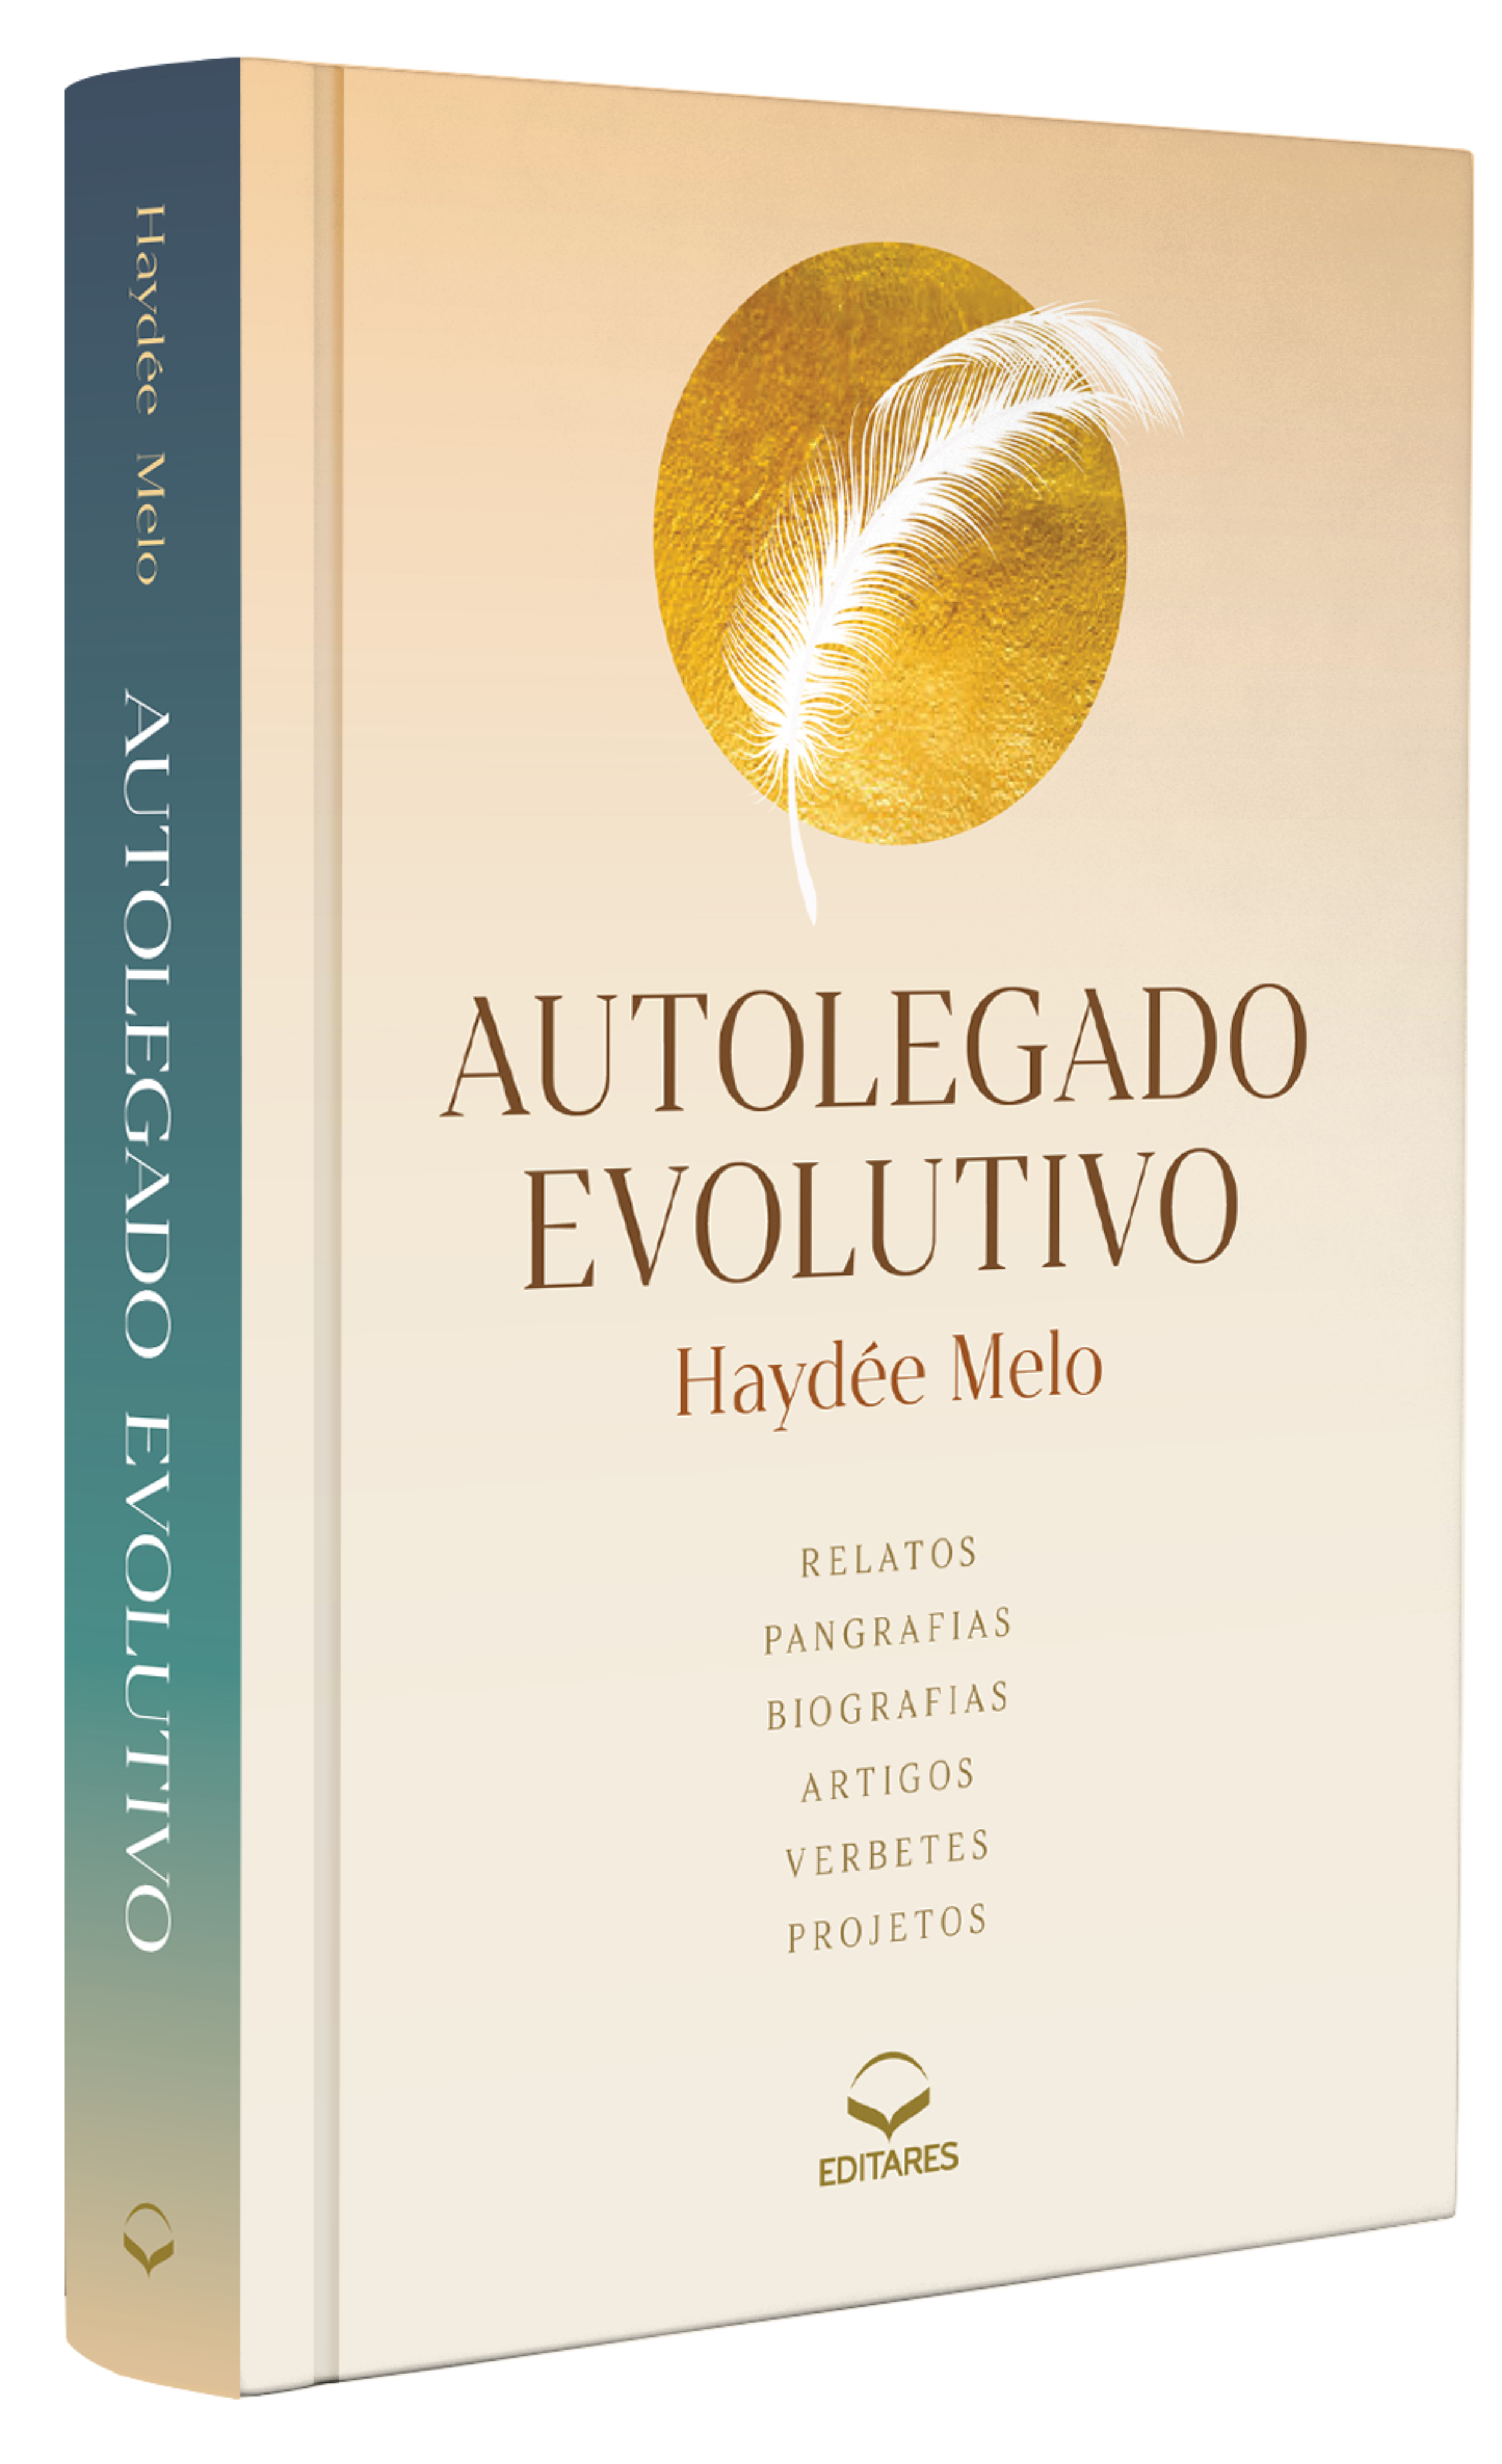
\includegraphics[width=5cm]{articles/entrevista/mockups/Haydee_Melo}
\end{center}


\textbf{1. Qual foi a~motivação para a~escrita da obra? Por que a~definição deste tema para publicação de um livro?}


Duas motivações foram a~mais importantes. Em primeiro lugar, reunir as principais gescons de Haydée de modo a~funcionar como cápsula do tempo para a~própria autora, a~ser reencontrado, reconhecido e~utilizado em vida futura. Fica muito mais fácil se as principais gestações estiverem reunidas em um só volume. Não menos importante, houve o~objetivo de assistir leitoras e~leitores interessados em Conscienciologia aplicada, a~exemplo dos vários projetos desenvolvidos pela autora em escolas e~na área de educação. O~livro também é~importante porque trata da história da própria Conscienciologia no planeta. Haydée foi líder do Instituto de Pesquisa da Consciência (IPC), instituição que foi reconhecida como parte da CCCI em 2003 e~que se uniu ao IIPC no mesmo ano. Cada seção da obra reconta importantes fatos e~parafatos, resgatando e~atualizando parte da holohistória dessa neociência para os próprios intermissivistas e~integrantes da maxiproéxis grupal.

\begin{pullquote}
``O livro também é~importante porque trata da história da própria Conscienciologia no planeta.''
\end{pullquote}

\subsubsection{2. Quais foram as principais percepções, intra e~extrafísicas, durante a~pesquisa e~a~escrita da obra? E~posterior ao lançamento?}


Muitas, principalmente relacionadas a~consciexes que tinham relação com o~IPC. Por um lado, notamos claramente aquela equipex presente, especialmente uma das consciências que lideraram o~IPC extrafisicamente e~que possui profunda relação de muitas vidas com Haydée. Por outro lado, ficou claro que este livro faz parte desse processo abrangente de união, antidiáspora, intra e~extrafísicos. Então, houve a~assistência também a~consciências que ainda não haviam feito a~transição completa à~CCCI. Posterior ao lançamento, a~interassistência a~esse movimento complexo continuou com a~segunda edição da obra, onde foram feitos alguns reajustes.


\textbf{3. Qual o~maior aprendizado com a~escrita desta obra?}

Um dos maiores aprendizados é~de que não existe obra simples do ponto de vista multidimensional. Todo e~qualquer livro, especialmente os de conteúdos pró-evolutivos, mexem com interrelações intricadas e~que muitas vezes só se tornam mais claras quando o~processo de escrita e~publicação ocorrem. Quando existe pré-disposição, tudo que está guardado vem à~tona e,~infalivelmente, precisará ser revisto e~reperspectivado. Ao mesmo tempo, livros conscienciológicos possuem um nível de interdependência diferenciados, onde o~que está sendo publicado afeta o~grupo como um todo. Tudo isso adiciona níveis de complexidade que somente quem é~autor ou parte do processo de publicação passa a~compreender.

\textbf{4. O~que poderia dizer como incentivo para que mais pesquisadores invistam na publicação de obras conscienciológicas?}

Essa obra foi fundamental para a~autora. Ela sempre dizia de que não poderia dessomar sem ter ao menos um livro publicado. Havia muita clareza de que tinha que retribuir tudo que recebeu e,~por isso, estava escrevendo o~tratado \emph{Homo sapiens neonatus,} repassado oficialmente para a~Evolucin. Esse livro, no meu ponto de vista, é~uma espécie de coroamento de uma vida dedicada à~interassistência, demonstrando quem essa consciência é~e~do que é~capaz. Eu também penso que existem muitas vias hoje em dia para a~publicação de um livro. A~reunião de gescons, por exemplo, pode ser uma das possibilidades, evidenciando a~evolução grafopensênica do autor ou autora.\\



% \begin{pullquote}
% ``Um dos maiores aprendizados é~de que não existe obra simples do ponto de vista multidimensional.''
% \end{pullquote}

    
    \end{multicols}
\end{document}
